\documentclass[11pt]{article}

\usepackage{amsmath}
\usepackage{amssymb}
\usepackage{booktabs}
\usepackage{float}
\usepackage{geometry}
\usepackage{graphicx}
\usepackage{hyperref}
\usepackage{xcolor}

\pdfminorversion=4
\pdfobjcompresslevel=0

\geometry{a4paper, margin=1in}
\setlength{\parindent}{0pt}

\title{BUSFIN 8200 -- Problem Set 2}
\author{Maeve Nguyen}
\date{\today}

\begin{document}
\maketitle

\section*{Question 1}

\section*{Question 2}
\subsection*{2 (a)}
Using the normalization $\mathbb{E}[M^*] = 1$, we find the stochastic discount factor $M_t^* = a - b'xR_t$ 
that satisfies $\mathbb{\hat{E}}[M^* \cdot xR] = 0$. In particular, we have:
\begin{align*}
    0 
    &= \mathbb{{E}}[M^* \cdot xR] \\
    &= \underbrace{\mathbb{{E}}[M^*]}_{\displaystyle = 1} \cdot \mathbb{E}[xR] + \text{Cov}(M^*, xR) \\
    &= \mathbb{E}[xR] - b'\text{Cov}(xR, xR) \\
    &\implies \mathbb{E}[xR] = b'\Sigma \\
    &\implies b = \Sigma^{-1}\mathbb{E}[xR] 
\end{align*}

$xR$ is a Tx10 vector of excess returns with T = 1,202 months in the sample from July 1926 to August 2026. Verifying that $\Sigma$ is invertible,
we find that:
\begin{align*}
    1 
    &= \mathbb{{E}}[M^*] \\
    &= \mathbb{E}[a - b'xR] \\
    &= a - b'\mathbb{E}[xR] \\
    &\implies a = 1 + b'\mathbb{E}[xR] \\
\end{align*}
Therefore, we are able to compute the stochastic discount factor $M_t^* = a - b'xR_t$ for each month in the sample and obtain the following scatterplot:
\begin{figure}[H]
    \centering
    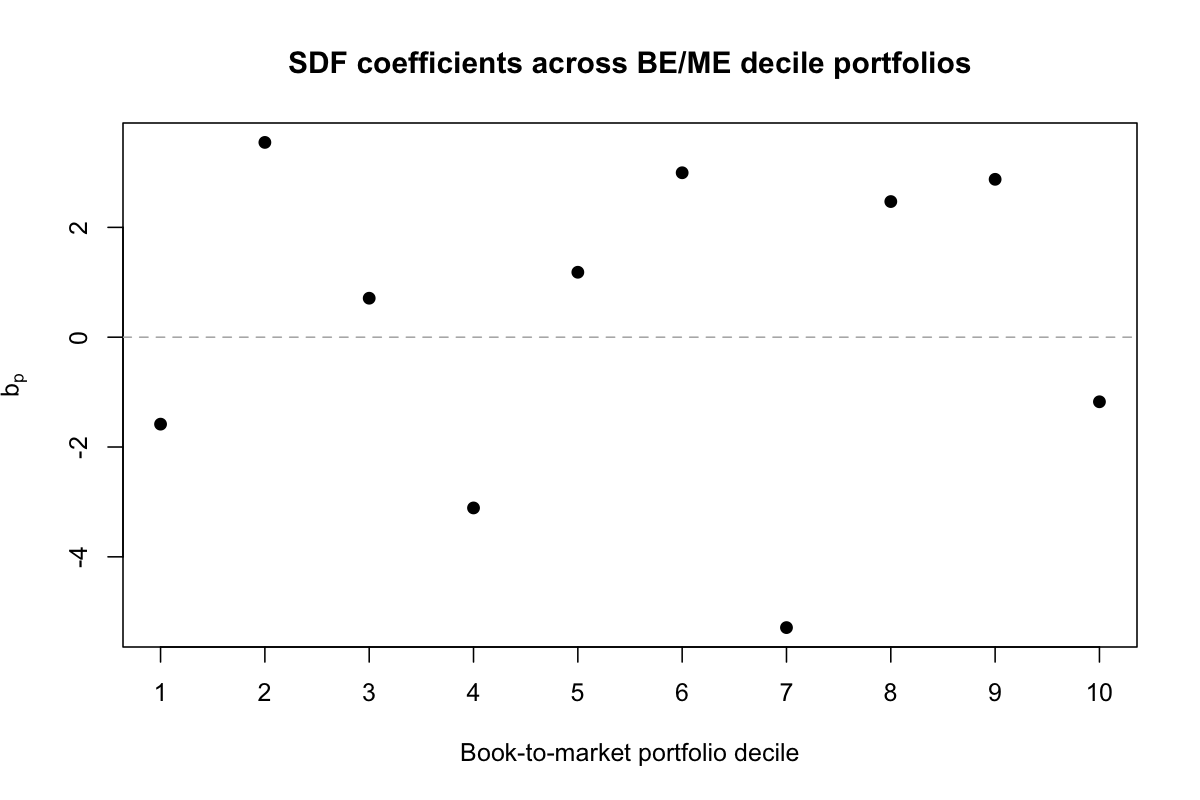
\includegraphics[width=0.6\textwidth]{figures/2a.png}
    \label{fig:q2a}
\end{figure}

\subsection*{2 (b)}
Following the same procedure as in part (a), we find the respective b coefficients of the stochastic discount factor that prices the excess returns of
the 10 portfolios in the $MOM$ dataset as follows: 
\begin{figure}[H]
    \centering
    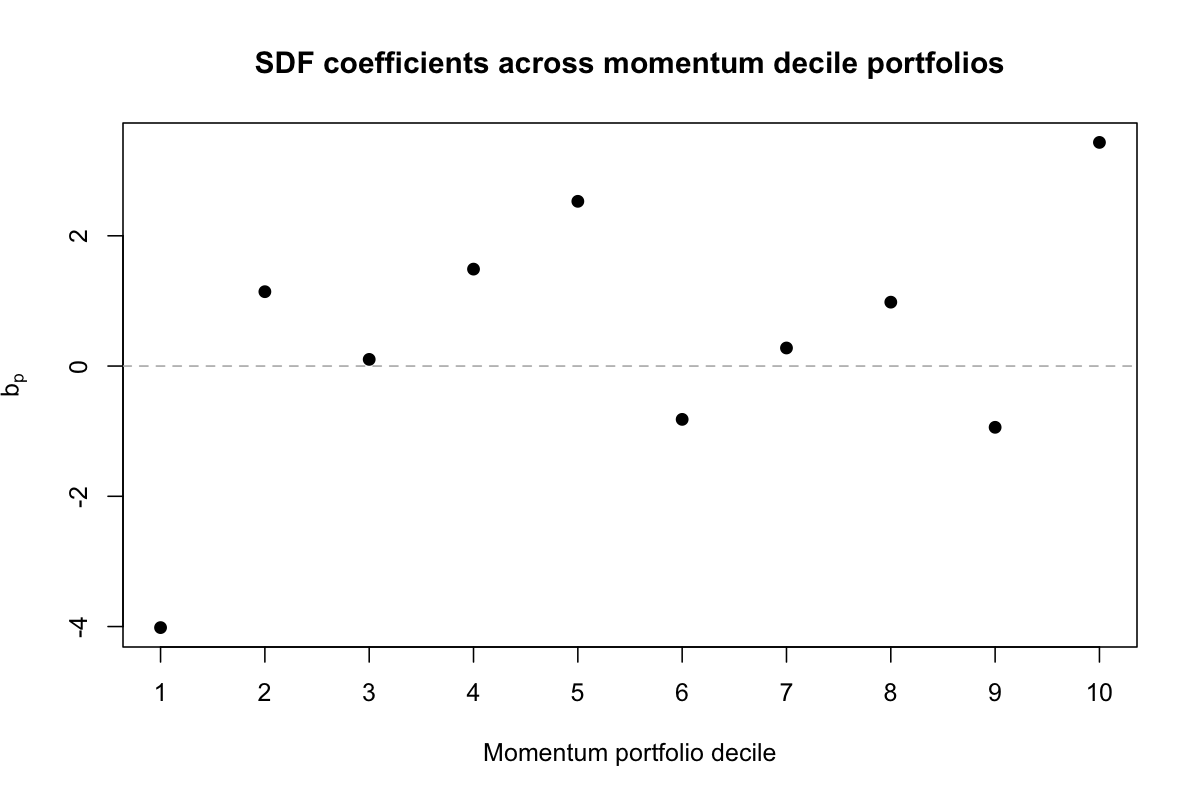
\includegraphics[width=0.6\textwidth]{figures/2b.png}
    \label{fig:q2b}
\end{figure}

Similar to part (a), we do not observe any clear pattern between the b coefficients and the decile portfolios' excess returns. 
The correlation between the recovered $M_t^*$ is 0.3555, which suggests that the SDF that prices a particular portfolio does not
necessarily price the other one as the decile portfolios are sorted using different signals. 

\subsection*{2 (c)}
Following the same procedure as in part (a), we find the respective b coefficients of the
stochastic discount factor that prices the excess returns of the 20 portfolios in the $BM$ \& $MOM$ datasets as follows:
\begin{figure}[H]
    \centering
    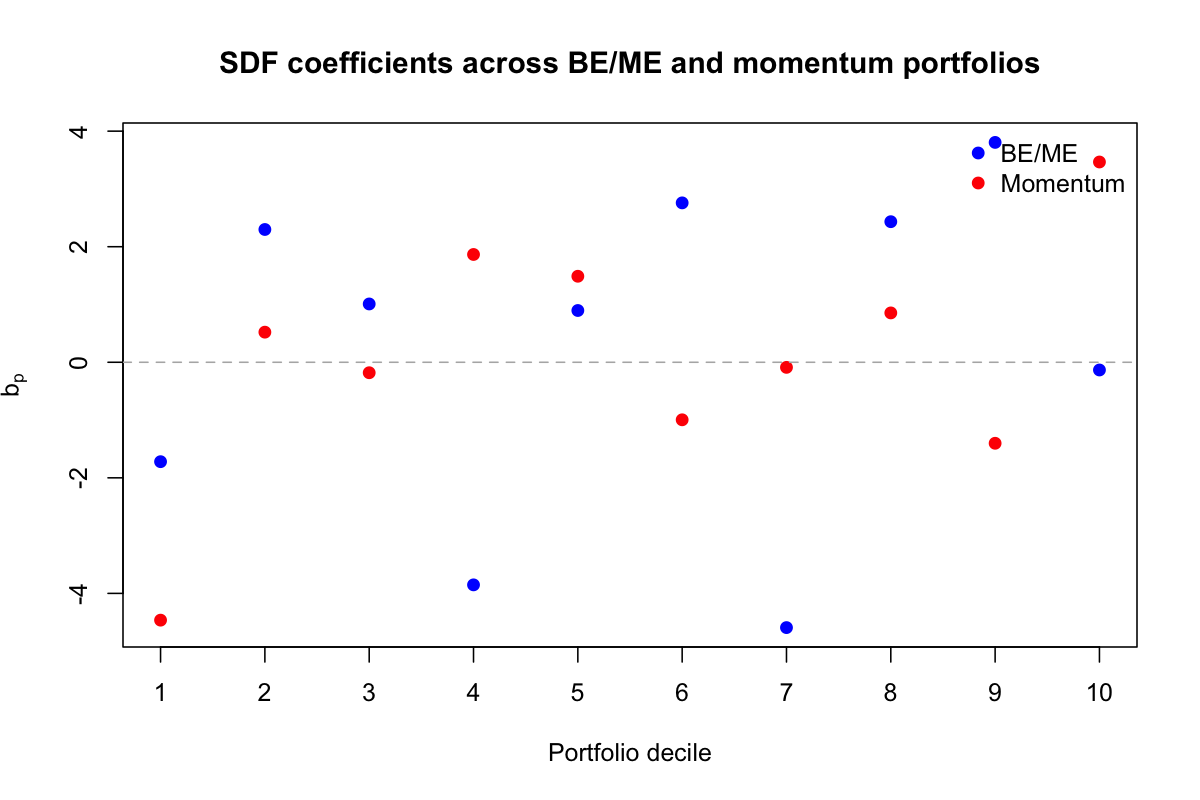
\includegraphics[width=0.6\textwidth]{figures/2c.png}
    \label{fig:q2c}
\end{figure}

Using a common sample of 1,196 months from July 1927 to August 2026, we estimated
the Sharpe ratios of $xR_t^*$ as follows: 
\begin{table}[H]
  \centering
  \caption{Monthly Sharpe Ratios of the $xR^*$ Portfolios}
  \label{tab:2c-sharpe-ratios}
  \begin{tabular}{lr}
    \toprule
    Portfolio set & Monthly Sharpe ratio \\
    \midrule
    BE/ME (10 portfolios) & 0.191841 \\
    Momentum (10 portfolios) & 0.257990 \\
    Combined (20 portfolios) & 0.304398 \\
    \bottomrule
  \end{tabular}
\end{table}

A key property of the SDF under no arbitrage is that $xR_t^*$ is the maximum Sharpe ratio portfolio. 
Since we observed that the Sharpe ratio of the combined 20 portfolios is higher than the Sharpe ratios of the individual 10 portfolios, 
adding more non-redundant assets to the portfolio universe provides a more diversified portfolio with better risk-adjusted returns and higher volatility, which
is consistent with the theory of SDF and maximum Sharpe ratio portfolios.

\subsection*{2 (d)}
Having estimated the SDFs $M_t^* = \hat{a} - \hat{b}'xR_t$ from part (a),(b), and (c) and normalizing $\mathbb{E}[M^*]=1$, we estimate the pricing errors for each decile portfolio p as follows: 
\[
\hat{\alpha}_p
=
\widehat{\mathbb{E}}[xR_p]
+
\widehat{\operatorname{Cov}}(M^*, xR_p).
\]

\begin{table}[H]
  \centering
  \caption{Pricing Errors Under the Three Estimated SDFs}
  \label{tab:2d-pricing-errors}
  \begin{tabular}{lrrr}
    \toprule
    Portfolio & BE/ME SDF & Momentum SDF & Combined SDF \\
    \midrule
    BE/ME D1 & 0.000005 & -0.001505 & 0.000005 \\
    BE/ME D2 & 0.000006 & -0.000095 & 0.000006 \\
    BE/ME D3 & 0.000006 & -0.000217 & 0.000006 \\
    BE/ME D4 & 0.000006 & -0.000772 & 0.000006 \\
    BE/ME D5 & 0.000006 & 0.000509 & 0.000006 \\
    BE/ME D6 & 0.000007 & 0.001267 & 0.000007 \\
    BE/ME D7 & 0.000006 & 0.000287 & 0.000006 \\
    BE/ME D8 & 0.000008 & 0.002382 & 0.000008 \\
    BE/ME D9 & 0.000009 & 0.003456 & 0.000009 \\
    BE/ME D10 & 0.000009 & 0.003204 & 0.000009 \\
    Momentum D1 & -0.010147 & 0.000001 & 0.000001 \\
    Momentum D2 & -0.005043 & 0.000004 & 0.000004 \\
    Momentum D3 & -0.003265 & 0.000004 & 0.000004 \\
    Momentum D4 & -0.001482 & 0.000005 & 0.000005 \\
    Momentum D5 & -0.000875 & 0.000006 & 0.000006 \\
    Momentum D6 & -0.000257 & 0.000006 & 0.000006 \\
    Momentum D7 & 0.000515 & 0.000006 & 0.000006 \\
    Momentum D8 & 0.001908 & 0.000007 & 0.000007 \\
    Momentum D9 & 0.002246 & 0.000008 & 0.000008 \\
    Momentum D10 & 0.005424 & 0.000010 & 0.000010 \\
    \bottomrule
  \end{tabular}
\end{table}

We observe that the SDF constructed using the BE/ME portfolios prices the BE/ME portfolios well with small pricing errors, 
but not the MOM portfolios, and vice versa. The SDF based on the combined 20 portfolios prices 
all 20 portfolios well, which is consistent with the notion that the selection of the asset universe
matters in the pricing power of the SDF. 

\subsection*{2 (e)}
Repeating the same procedure as in part (c) but restricting the sample to December 1989, I re-estimate $\hat{a}_{OS}= 1.12459$ 
and corresponding $\hat{b}_{OS}$ coefficients for the SDF that prices the 20 portfolios in the $BM$ \& $MOM$ datasets.
Then, using out-of-sample $xR_t$ from January 1990 to August 2026, I construct $M_{OS,t}^* = \hat{a}_{OS} - \hat{b}_{OS}'xR_t$ and 
obtain the following pricing errors:

\begin{table}[H]
  \centering
  \caption{Out-of-Sample Pricing Errors}
  \label{tab:2e-pricing-errors}
  \begin{tabular}{lr}
    \toprule
    Portfolio & OS pricing error \\
    \midrule
    BE/ME D1 & 0.010968 \\
    BE/ME D2 & 0.007859 \\
    BE/ME D3 & 0.009001 \\
    BE/ME D4 & 0.006958 \\
    BE/ME D5 & 0.007985 \\
    BE/ME D6 & 0.007179 \\
    BE/ME D7 & 0.006975 \\
    BE/ME D8 & 0.005926 \\
    BE/ME D9 & 0.008271 \\
    BE/ME D10 & 0.009709 \\
    Momentum D1 & 0.027023 \\
    Momentum D2 & 0.016469 \\
    Momentum D3 & 0.013896 \\
    Momentum D4 & 0.012071 \\
    Momentum D5 & 0.009178 \\
    Momentum D6 & 0.008297 \\
    Momentum D7 & 0.007601 \\
    Momentum D8 & 0.006446 \\
    Momentum D9 & 0.004326 \\
    Momentum D10 & 0.005462 \\
    \bottomrule
  \end{tabular}
\end{table}

Contrary to the in-sample results, the out-of-sample pricing errors are much larger, even for the
combined SDF, which suggests the possibility of time-varying $a$ and $b$ coefficients in the SDF. 

\section*{Question 3}
\subsection*{3 (a)}
Consider a representative investor with wealth $W_t$ in a two-period economy. Let
$R_{f,t}$ be a baseline asset. We solve the following optimization problem:
\begin{align*}
    \mathbf{w}_t^*
    &= \arg\max_{\mathbf{w}_t} \mathbb{E}_t\!\left[U(W_{t+1})\right], \\
    \text{s.t.}\quad
    W_{t+1}
    &= W_t R_{m,t+1}
     = W_t\left(R_{f,t+1}+\mathbf{w}_t' xR_{t+1}\right),
\end{align*}
where $xR_{t+1}$ is the vector of asset excess returns relative to $R_{f,t}$.

Using the power utility function
\[
    U(W)=\frac{W^{1-\gamma}}{1-\gamma},
\]
where $\gamma$ is CRRA, we rewrite the problem as
\[
    \mathbf{w}_t^*
    = \arg\max_{\mathbf{w}_t}
      \mathbb{E}_t\!\left[
        \frac{
          \left(W_t\left(R_{f,t+1}+\mathbf{w}_t' xR_{t+1}\right)\right)^{1-\gamma}
        }{1-\gamma}
      \right].
\]

Thus, the first-order condition of the maximization problem is
\begin{align*}
    \mathbb{E}_t\!\left[
      \frac{
        (1-\gamma)W_t
        \left(R_{f,t+1}+\mathbf{w}_t' xR_{t+1}\right)^{-\gamma}
        xR_{t+1}
      }{1-\gamma}
    \right] &= 0 \\
    \implies
    \mathbb{E}_t\!\left[
      \left(R_{f,t+1}+\mathbf{w}_t' xR_{t+1}\right)^{-\gamma}
      xR_{t+1}
    \right] &= 0 \\
    \implies
    \mathbb{E}_t\!\left[
      R_{m,t+1}^{-\gamma}xR_{t+1}
    \right] &= 0.
\end{align*}
As a result, the SDF $M_t=R_{m,t+1}^{-\gamma}$ prices the vector of excess returns.

\subsection*{3 (b)}

\subsection*{3 (c)}

\subsection*{3 (d)}

\subsection*{3 (e)}

\section*{Question 4}
\subsection*{4 (a)}

\subsection*{4 (b)}

\subsection*{4 (c)}

\subsection*{4 (d)}

\subsection*{4 (e)}

\end{document}

